\documentclass[fontset=windows]{article}
\usepackage[margin=1in]{geometry}
\usepackage{ctex}
\usepackage{setspace}
\usepackage{lipsum}
\usepackage{graphicx}
\usepackage{caption}
\usepackage{subcaption}
\usepackage[colorlinks=true,linkcolor=red]{hyperref}

\graphicspath{{figures/}}

\title{\heiti\zihao{2} MOS Small-Signal Model, PMOS Device}
\author{\songti zrrraa}
\date{2023.11.17}

\begin{document}
\maketitle
\thispagestyle{empty}

\section*{Large-Signal \& Small-Signal Operation}

\begin{figure}[htbp]
    \centering
    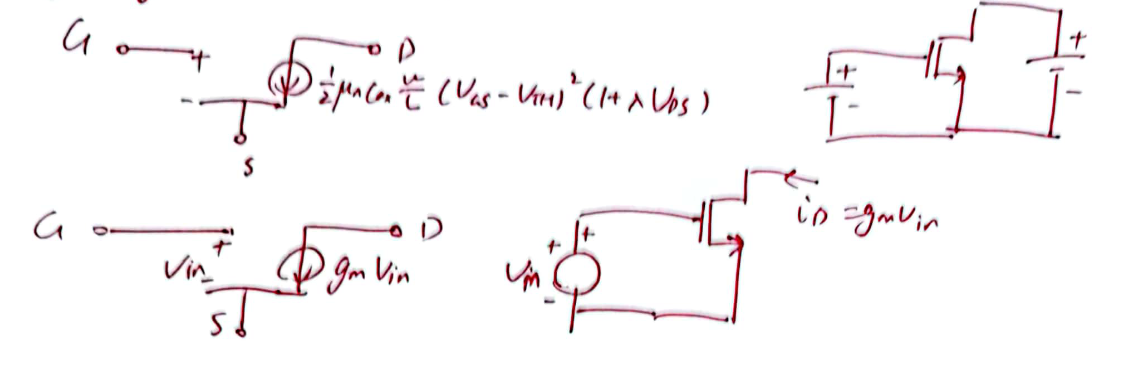
\includegraphics[scale=0.6]{1.jpg}
    \captionsetup{labelformat=empty}
    \caption{Large-Signal \& Small-Signal Operation}
    \label{1}
\end{figure}

\section*{Small-Signal Models of Const Sources}

In const sources, we make all constants equal 0. 

\begin{figure}[htbp]
    \centering
    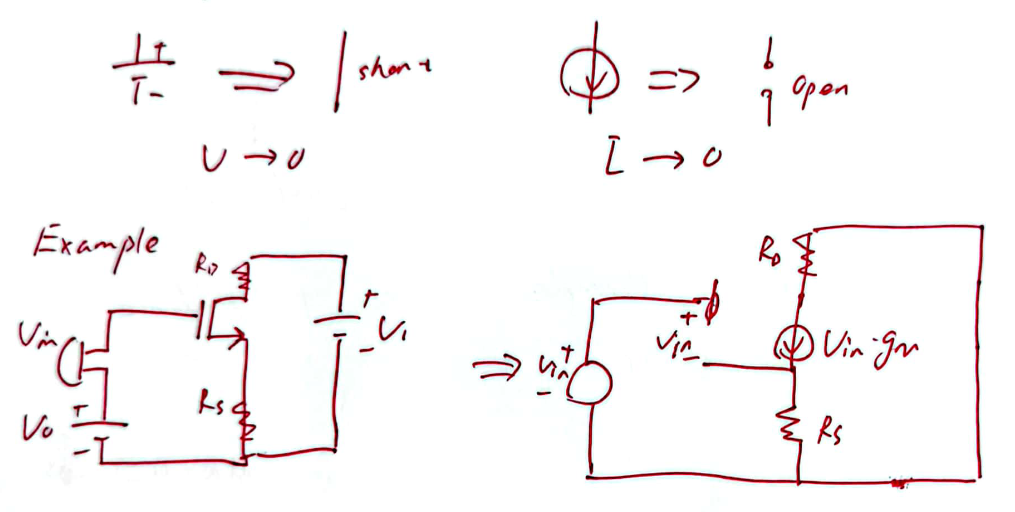
\includegraphics[scale=0.6]{2.jpg}
    \captionsetup{labelformat=empty}
    \caption{Small-Signal Models of Const Sources}
    \label{2}
\end{figure}

Here's a example. 

\begin{figure}[htbp]
    \centering
    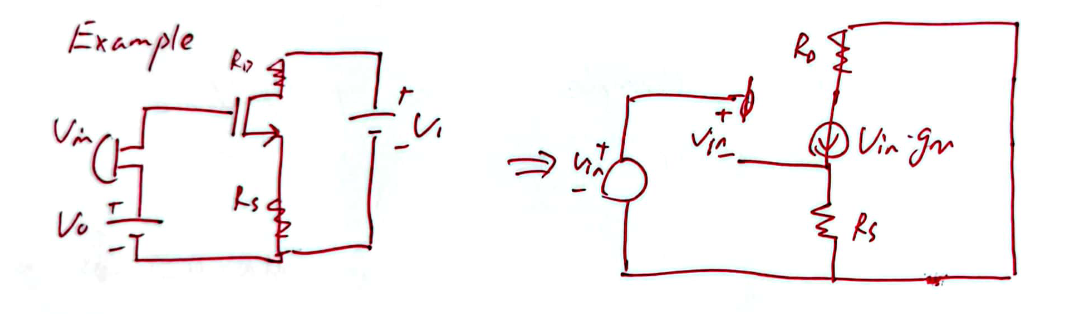
\includegraphics[scale=0.6]{3.jpg}
    \captionsetup{labelformat=empty}
    \caption{}
    \label{3}
\end{figure}

\section*{General Procedure of Constructing a Small-Signal Model}

\begin{itemize}
	\item Apply proper bias voltages to the device. 
	\item Increment the voltage difference between two terminals. 
	\item Measure all current increments. 
	\item Model the change by a proper electrical device. 
\end{itemize}

\begin{figure}[htbp]
    \centering
    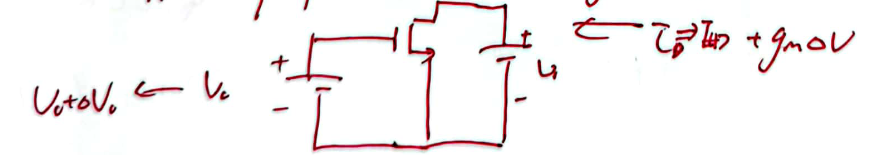
\includegraphics[scale=0.6]{4.jpg}
    \captionsetup{labelformat=empty}
    \caption{Increment of $V_{GS}$}
    \label{4}
\end{figure}

In the second point above, we want to study the effect of the voltage increment at the two terminals on the circuit. 
Let's take a look at the impact of increasing $V_{DS}$ on the circuit. 

$$I_D=\frac{1}{2} \mu_n C_{ox}\frac{W}{L}(V_{GS}-V_{TH})^2(1+\lambda V_{DS})$$

Now we take consideration of the Channel-Length Modulation, so the increment of $V_{DS}$ leads to the increment of $I_D$. 

$$I_D+\Delta I_D=\frac{1}{2} \mu_n C_{ox}\frac{W}{L}(V_{GS}-V_{TH})^2(1+\lambda V_{DS}+\lambda \Delta V_{DS})$$

$$I_D+\Delta I_D=I_D+\frac{1}{2} \mu_n C_{ox}\frac{W}{L}(V_{GS}-V_{TH})^2\lambda \Delta V_{DS}$$

Here we  regard $\frac{1}{2} \mu_n C_{ox}\frac{W}{L}(V_{GS}-V_{TH})^2$ approximately as $I_D$. 

So we can get: 

$$\frac{\Delta V_{DS}}{\Delta I_D}\approx \frac{1}{\lambda I_D}=r_o$$

We think of the connection between drain and source as a resistor. 

\begin{figure}[htbp]
    \centering
    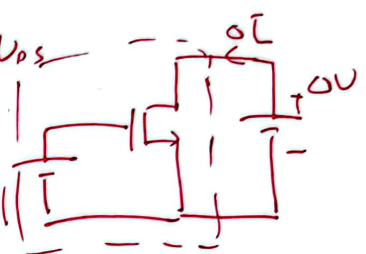
\includegraphics[scale=0.6]{5.jpg}
    \captionsetup{labelformat=empty}
    \caption{Think of the connection between drain and source as a resistor}
    \label{5}
\end{figure}

Neglect the effect of Channel-Length Modulation on the $g_m$ expressions. 
Here's the small-signal model with $r_o$. 

\begin{figure}[htbp]
    \centering
    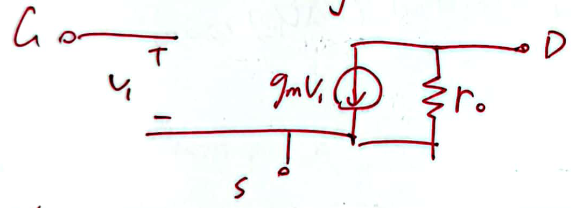
\includegraphics[scale=0.6]{6.jpg}
    \captionsetup{labelformat=empty}
    \caption{Small-Signal model with $r_o$}
    \label{6}
\end{figure}

\subsection*{Example}

\begin{figure}[htbp]
    \centering
    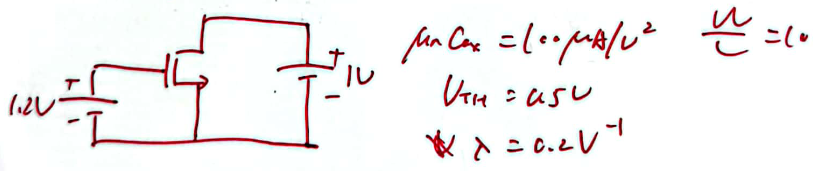
\includegraphics[scale=0.6]{7.jpg}
    \captionsetup{labelformat=empty}
    \caption{}
    \label{7}
\end{figure}

$$V_{GS}-V_{TH}\leq V_{DS}\Longrightarrow Saturation$$

$$I_D=\frac{1}{2} \mu_n C_{ox}\frac{W}{L}(V_{GS}-V_{TH})^2\Longrightarrow r_o=\frac{1}{\lambda I_D}\Longrightarrow r_o=20.4k\Omega$$

$$g_m=\mu_n C_{ox}\frac{W}{L}(V_{GS}-V_{TH})=\frac{1}{1.43k\Omega}$$

\section*{PMOS}

\begin{figure}[htbp]
    \centering
    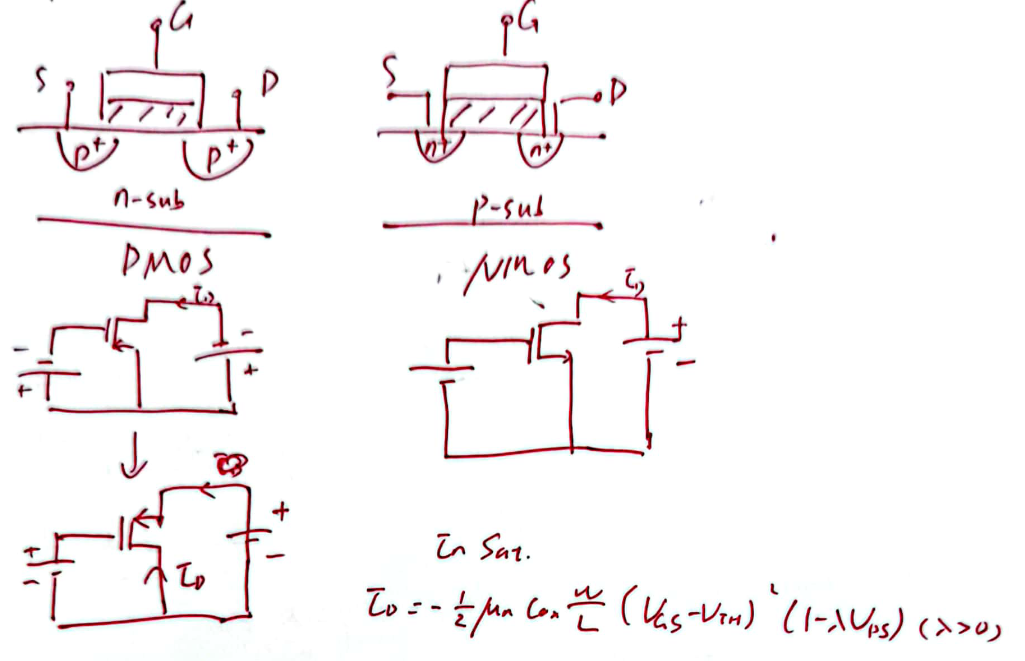
\includegraphics[scale=0.6]{8.jpg}
    \captionsetup{labelformat=empty}
    \caption{}
    \label{8}
\end{figure}

For PMOS: 

\begin{itemize}
    \item $V_G<V_S$
    \item $V_{TH}<0$
    \item $V_D<V_S$
\end{itemize}

In PMOS, the Gate voltage is minus, so it can attract the holes to form the channel. 
The current flows from Source to Drain. 

\subsection*{Large-Signal Model}

Pay attention, $I_D$ is still defined from Drain to Source. So it's minus. 

\begin{figure}[htbp]
    \centering
    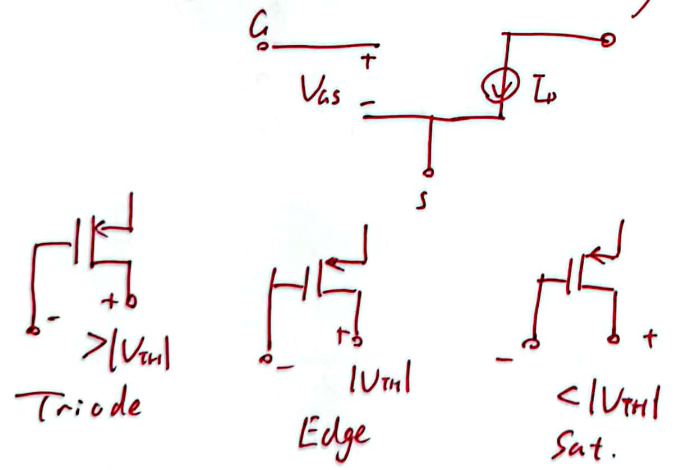
\includegraphics[scale=0.5]{9.jpg}
    \captionsetup{labelformat=empty}
    \caption{}
    \label{9}
\end{figure}

\subsection*{Small-Signal Model}

\begin{figure}[htbp]
    \centering
    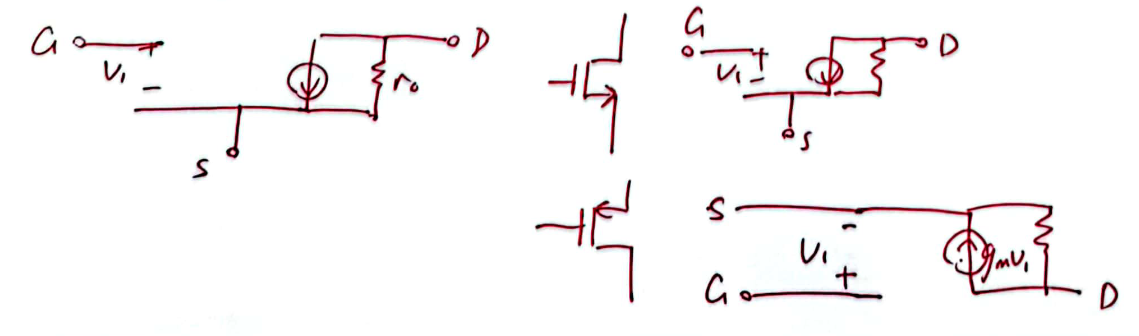
\includegraphics[scale=0.45]{10.jpg}
    \captionsetup{labelformat=empty}
    \caption{}
    \label{10}
\end{figure}

\section*{Link}

\href{https://www.bilibili.com/video/BV1FD4y1R7Ah?p=34&vd_source=1d0c07486a3bd3b0adb8ac548bf6453e}{Razavi Electronics Circuits 1: lectrue 34}
\end{document}